\begin{figure*}[t!]
\centering
%\missingfigure{$P_N$-solver overview: generate stencil code $\rightarrow$ build system $\rightarrow$ solve $\rightarrow$ render}
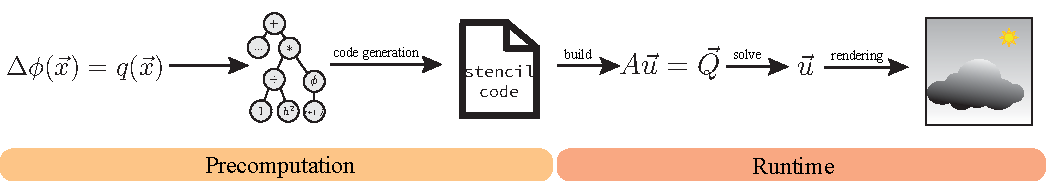
\includegraphics[width=\textwidth]{figures/fig_pipeline.pdf}
\vspace{-0.2in}
\icaption{Overview of our $P_N$-solver. After generating the stencil source code from the expression trees representing the $P_N$-equations, the linear system $A\vec{u}=\vec{Q}$ is built using RTE parameter fields and additional user input, such as grid resolution and type of boundary conditions. The resulting system is solved for $\vec{u}$, which is then used in our rendering application.}
\label{fig:pnsolver}
\end{figure*}

\vspace{-0.75in}

\section{$P_N$-Solver}
\label{sec:pnsolver}

The truncation order $N$ is the key input parameter to the solver. With higher values, manual implementation of the solver from the equations would be ardous, error-prone and time-consuming. We therefore decided to make use of the computer algebra representation and designed our solver around it.

The solver consists of two components. The first is a precomputation (Section~\ref{sec:solver_precomputation}), which is excuted once for every single value of $N$. This steps runs a partial evaluation on the mathematical expression tree and applies the spatial discretization in a reference space we call stencil space. The precomputation step automatically generates source code from the resulting expression tree.

The generated stencil code is compiled with the runtime component (Section~\ref{sec:solver_runtime}) of our solver. This component receives the actual problem as input, including grid resolution and RTE parameter fields. It then builds the linear system and solves it using standard methods. An overview of the solver is given in Figure~\ref{fig:pnsolver}.



\subsection{Precomputation}
\label{sec:solver_precomputation}

The result of the precomputation is a stencil, which can be used during runtime to build the linear system for a given problem. The stencil is a pattern of indices into the solution vector, along with values. It expresses how the sum of the weighted solution vector, components relate to the RHS for a given unknown in the system and therefore contains most information required to fill the system matrix $A$ and RHS-vector $\vec{Q}$ row by row. Note that while the coefficients may change, the sparsity pattern of the stencil is identical for different rows.

\begin{figure}[b]
\centering
%\missingfigure{test}
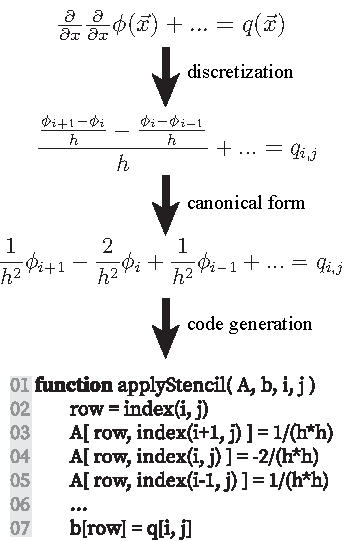
\includegraphics[width=0.7\columnwidth]{figures/fig_stencil_pipeline.pdf}
%\vspace{-0.2in}
\icaption{Creating the stencil code requires several steps, usually done by hand. We express the given problem in a computer algebra representation and use it to fully automate the process.}
\label{fig:stencile_pipeline}
\end{figure}

\vspace{0.6in}

Stencil generation entails discretizing a PDE at a hypothetical center voxel $(i, j, k)$ (assuming to mean the voxel center most of the time). Finite differences create weighted references to other voxels (e.g. $i+1, j, k$). After bringing the discretized equation into canonical form (a weighted sum of unknowns), one can write the stencil by reading off the weights and offsets (Figure~\ref{fig:stencile_pipeline}). $(i, j, k)$ will only be known during runtime, when the stencil is executed for a particular unknown (row). Then the offsets can be used to find the component index into the solution-vector, and weights can be evaluated for concrete world space position. We refer to the space with the hypthetical voxel $(i, j, k)$ at the center as stencil space.

\vspace{0.2in}

\begin{wrapfigure}{r}{0.6\columnwidth}
%\begin{center}
\hspace{-.2in}
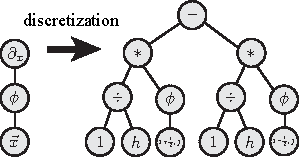
\includegraphics[width=0.6\columnwidth]{figures/fig_discretization.pdf}
%\end{center}
\end{wrapfigure}The spatial discretization is done by parsing the expression tree from the root. The discrete substitute for the continuous position variable $\vec{x}$ is initialized with $ijk$. Differential operator nodes are replaced by a subtree, which expresses the finite difference approximation (including voxelsize factor $h$). The subtree of the differential operator node is duplicated for different offsets to the discrete variable $(i, j, k)$. Since this offset only applies to the substree, a stack is maintained by the parser to manage scope. Whenever the parser encounters the continuous variable $\vec{x}$ in the expression tree, its node in the tree is replaced by the discrete substitute, currently on top of the stack. Nested differential operators yield higher order finite difference stencils as expected.

\begin{wrapfigure}{r}{0.6\columnwidth}
%\begin{center}
\hspace{-.2in}
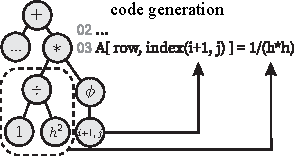
\includegraphics[width=0.6\columnwidth]{figures/fig_codegen.pdf}
%\end{center}
\end{wrapfigure}
Factorization into canonical form is done as a manipulation pass on the mathematical expression tree. The result allows to implement the code generation in a straight forward fashion. For each term, the $ijk$-offset is retrieved from the unknown. The factor-expression, which is multipled with the unknown, is extracted from the tree and used to generate source code for evaluating the factor-expression during runtime (including calls for evaluating RTE-parameter fields).

\begin{figure}[h]

%\vspace{1in}
\centering
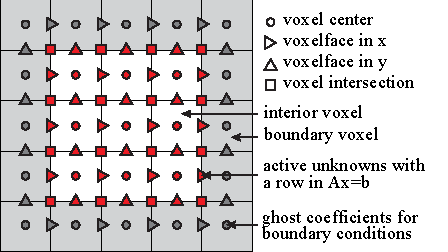
\includegraphics[width=0.9\columnwidth]{figures/fig_staggered_grids.pdf}
%\vspace{-0.2in}
\icaption{Staggered grids place coefficients at different locations within the finite difference grid.}
\label{fig:staggeredgrid}
\end{figure}

\begin{wrapfigure}{r}{0.6\columnwidth}
%\begin{center}
\hspace{-.1in}
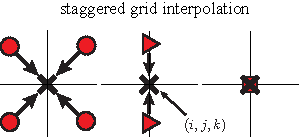
\includegraphics[width=0.6\columnwidth]{figures/fig_staggered_interpolation.pdf}
\vspace{-.1in}
%\end{center}
\end{wrapfigure}Our solver supports placement of coefficients at arbitrary staggered grid locations (see Figure~\ref{fig:staggeredgrid}). This means, that during the discretization step, the discrete location $(i, j, k)$ (at which the unknown is meant to be evaluated) might not coincide with the location of the unknown. To solve this, depending on how the two are located to each other, the parser returns an expression, which interpolates the coefficients at $(i, j, k)$ from their defined locations. If those happen to coincide, the coefficient itsself is returned. This is also done for RTE parameters, such as $\sigma_t$ or $p^{l,m}$, which are always located at the voxel center.


%\subsection{Stencil Code Generation}

% After applying the discretization step to the expression tree of the $P_N$-equations, it is used to generate the stencil code. In numerical analysis, a stencil is an arrangement of voxels and weights, that relate values at different locations to each other and form the basis for propagating rows in the system matrix $A$ and RHS vector $\vec{Q}$ with values. The name comes from the fact, that the geometric structure and weights of the configuration do not change, when applied to different voxels. The same is true for the $P_N$-equations and we use this fact to generate a single function, which propagates rows in $A$ and $\vec{Q}$ for a given voxel.

%The $P_N$-equations express, how each coefficient of a voxel depends on other coefficients of the same or adjacent voxels. The unknowns in the terms give information about the coefficient index and voxel offset, and therefore identify a column offset in the matrix $A$. The factors to these coefficients may contain evaluations of RTE parameters, such as $\sigma_t$. Therefore, these factors can not be determined during stencil generation, but are rendered into code expressions, which are executed as part of the stencil function during runtime. Because the stencil code has been generated in stencil space relative to the voxel at $(0,0,0)$, we can run the same stencil code for every voxel, by simply applying an offset accordingly. 



%\subsection{System Building and Solving}
\subsection{Runtime}
\label{sec:solver_runtime}

The stencil code is generated once for every value of $N$ and compiled with the runtime component of our solver. The runtime executes the stencil for every voxel to propagate the system matrix $A$ and RHS vector $\vec{Q}$ with numerical values.

The number of rows is determined by the number of voxels times the number of coefficients per voxel (see Figure~\ref{fig:matrix_layout}) and can therefore become very large for high resolution and high truncation order. The matrix $A$ is square and extremely sparse, due to the local structure of the finite differences discretization. Unfortunately, it is non-symmetric due to the transport term and not diagonal dominant, which rules out many \rev{iterative} methods for solving linear systems. \rev{Iterative methods are useful, as they allow balancing accuracy against performance by tweaking the convergence threshold.} We adress this by solving the normal form $A^TA\vec{u}=A^T\vec{Q}$ instead. This gives a symmetric and positive definit system matrix $A^TA$, albeit with a higher condition number. Investigation of other solution schemes (e.g. multigrid) would be an interesting avenue for future work. \rev{However, more importantly, in the presence of vacuum regions, the matrix $A$ becomes singular and the system cannot be solved at all. This requires the introduction of a minimum threshold for the extinction coefficient $\sigma_t$.}

Our solver supports Neumann and Dirichlet boundary conditions. They are handled transparently by the code which generates the stencil. Whenever the stencil accumulates coefficients into a boundary location, the framework either ignores the write operation (Dirichlet BC) or accumulates into the row and column in $A$ of the coefficient in the closest voxel inside the domain (Neumann BC). This is done changing the index of the written component under the hood.

%To respect the boundary correctly, additional coefficients (which contribute additional rows and columns in $A$ and $\vec{Q}$) are necessary at boundary voxels. This requires careful managegment and bookkeeping of coefficient indices, which is done transparently by the runtime code.





%\begin{figure}[h]
%\centering
%\begin{subfigure}{0.45\columnwidth}
%%\missingfigure{test}
%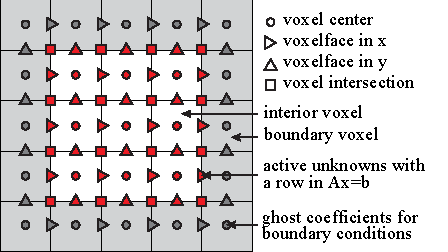
\includegraphics[width=\columnwidth]{figures/fig_staggered_grids.pdf}
%\end{subfigure}%
%\hspace{0.05\columnwidth}
%\begin{subfigure}{0.45\columnwidth}
%\missingfigure{test2}
%\end{subfigure}%
%\vspace{-0.2in}
%\icaption{Staggered grids cause a shifted boundary on the right and upper side of the domain (left). The boundary is correct after introducing additional unknowns (red) at boundary voxels (right).}
%\label{fig:staggeredgrid}
%\end{figure}


%Matrix $A$ and vector $\vec{Q}$ are constructed after applying the stencil for every voxel.



%\subsection*{CDA vs. $P_1$}
%\begin{itemize}
  %\item CDA is a degenerated form of $P_1$. It is derived by isolating the flux-vector on one side of the vector-equation formed by the $l=1$ SH-band equations. This isolation requires division by the extinction coefficient, introducing a $\frac{1}{\sigma_t}$ factor which diverges as $\sigma_t$ approaches zero. Thresholding to some minimum is required, in order to be able to solve the system for vacuum regions.
  %\item $P_1$ does not require any thresholding of $\sigma_t$ as it does not contain $\sigma_t$ as a denominator. It therefore can deal with vacuum regions without modifications.
  %\item (needs validation) Further, in the presence of vacuum or near vacuum regions, the condition number for CDA is higher than for $P_1$, because of small extinction values in the denominator of the diffusion coefficient.
  %\item Using the normal form for CDA will further increase the condition number when vacuum regions are present and significantly decreases convergence.
%\end{itemize}

